\documentclass[tikz,border=0pt]{standalone}

\usepackage{fontspec}
\defaultfontfeatures{Ligatures=TeX}
\setmainfont{Arial}
\setsansfont{Arial}
\renewcommand{\familydefault}{\sfdefault}

\usepackage{amsmath,amssymb,bm}
\usepackage[italic]{mathastext}
\usepackage{tikz}
\usetikzlibrary{arrows.meta,calc,fit,positioning,shapes.geometric}

\definecolor{FigBlue}{HTML}{2C78D0}
\definecolor{FigGreen}{HTML}{2E8B57}
\definecolor{FigOrange}{HTML}{C96A00}
\definecolor{FigRed}{HTML}{C74A44}
\definecolor{FigDark}{HTML}{202020}
\definecolor{FigGrid}{HTML}{D9D9D9}
\definecolor{FigLight}{HTML}{F4F4F4}
\definecolor{FigActorFill}{HTML}{F6F9FC}
\definecolor{FigFormulaFill}{HTML}{FCF8F6}

\newcommand{\RThreeTitle}{\fontsize{8.9}{9.8}\selectfont\bfseries}
\newcommand{\RThreeText}{\fontsize{7.35}{8.0}\selectfont}
\newcommand{\RThreeSmall}{\fontsize{6.75}{7.35}\selectfont}
\newcommand{\RThreeTiny}{\fontsize{6.25}{6.9}\selectfont}
\newcommand{\RThreeFormula}{\fontsize{6.85}{7.45}\selectfont}
\newcommand{\RThreeTerminal}{\fontsize{8.1}{8.9}\selectfont\bfseries}

\tikzset{
  r3base/.style={
    draw=FigDark,
    fill=FigLight,
    line width=0.9pt,
    align=center,
    inner sep=2.2pt,
    text=FigDark,
    font=\RThreeText
  },
  flowbox/.style={r3base, rectangle, draw=FigBlue, font=\RThreeTiny},
  stepbox/.style={r3base, rectangle, draw=FigGreen, fill=white},
  neutralbox/.style={r3base, rectangle, draw=FigGrid, fill=white},
  actorbox/.style={r3base, rectangle, draw=FigBlue, fill=FigActorFill},
  targetbox/.style={actorbox, dashed, line width=0.9pt},
  formulabox/.style={r3base, rectangle, draw=FigOrange, fill=FigFormulaFill},
  terminalbox/.style={
    r3base,
    ellipse,
    draw=FigBlue,
    fill=white,
    line width=1.0pt,
    font=\RThreeTerminal
  },
  decisionbox/.style={
    r3base,
    diamond,
    aspect=2.25,
    draw=FigOrange,
    fill=white,
    line width=1.0pt,
    inner sep=0.8pt,
    font=\RThreeTiny
  },
  outercallout/.style={
    draw=FigRed,
    dashed,
    line width=0.9pt,
    rounded corners=1pt,
    fill=none
  },
  mainarrow/.style={
    -{Latex[length=1.55mm,width=0.95mm]},
    draw=FigDark,
    line width=1.0pt,
    shorten >=4.0pt,
    shorten <=2.0pt
  },
  subarrow/.style={
    -{Latex[length=1.45mm,width=0.90mm]},
    draw=FigDark,
    line width=0.85pt,
    shorten >=3.5pt,
    shorten <=2.0pt
  },
  softarrow/.style={
    -{Latex[length=1.45mm,width=0.90mm]},
    draw=FigDark,
    dashed,
    line width=0.85pt,
    shorten >=3.5pt,
    shorten <=2.0pt
  },
  arrowlabel/.style={
    fill=white,
    inner sep=1.0pt,
    text=FigDark,
    font=\RThreeTiny
  }
}


\begin{document}
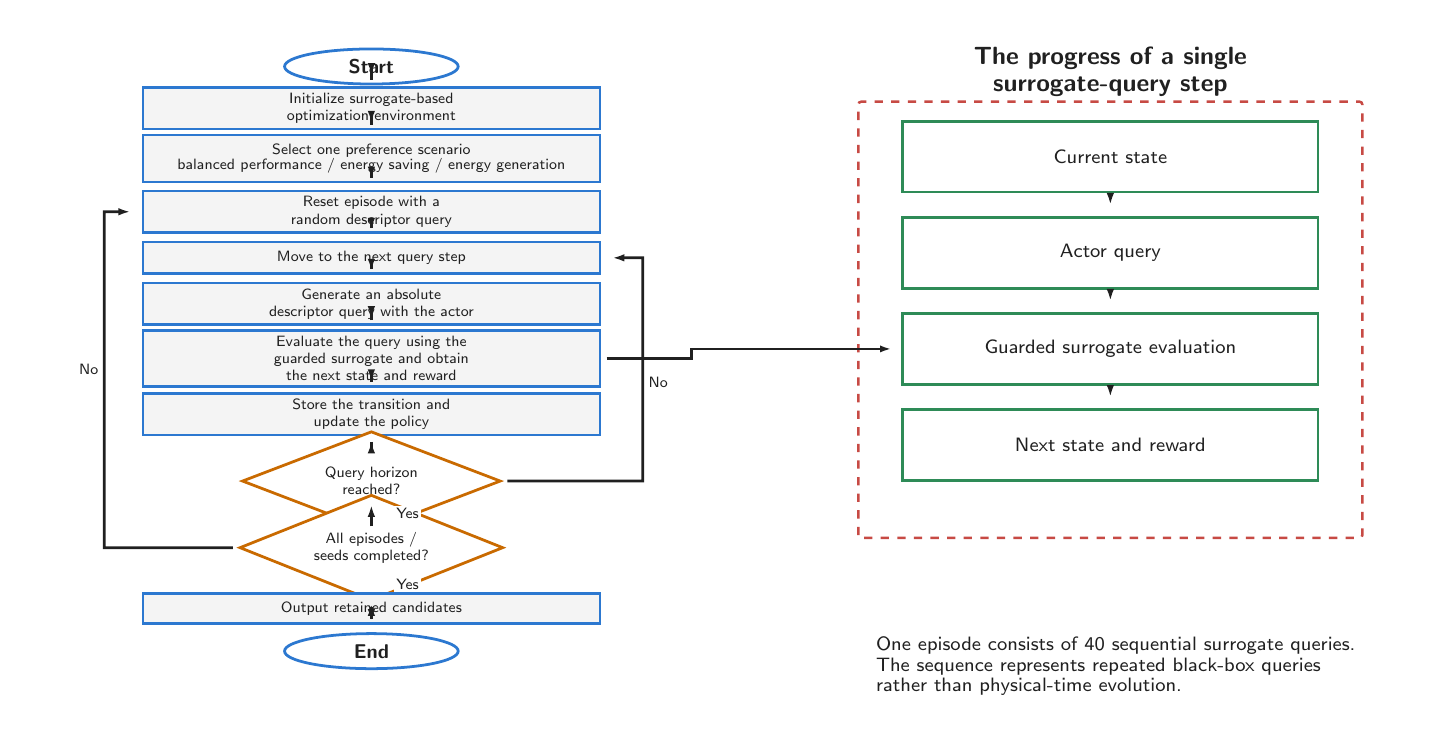
\begin{tikzpicture}[x=1cm,y=1cm]
\path[use as bounding box] (0,0) rectangle (17.5,8.8);

\begin{scope}[xshift=0.45cm,yshift=0.72cm,scale=0.90,transform shape]
\coordinate (mainX) at (4.35,0);
\node[terminalbox, minimum width=2.45cm, minimum height=0.38cm] (start) at (4.35,8.43) {Start};
\node[flowbox, minimum width=6.45cm, minimum height=0.50cm, text width=6.04cm] (init) at (4.35,7.84)
  {Initialize surrogate-based\\optimization environment};
\node[flowbox, minimum width=6.45cm, minimum height=0.66cm, text width=6.04cm] (scenario) at (4.35,7.13)
  {Select one preference scenario\\[-1pt]{\RThreeTiny balanced performance / energy saving / energy generation}};
\node[flowbox, minimum width=6.45cm, minimum height=0.52cm, text width=6.04cm] (reset) at (4.35,6.38)
  {Reset episode with a\\random descriptor query};
\node[flowbox, minimum width=6.45cm, minimum height=0.44cm, text width=6.04cm] (move) at (4.35,5.73)
  {Move to the next query step};
\node[flowbox, minimum width=6.45cm, minimum height=0.54cm, text width=6.04cm] (generate) at (4.35,5.08)
  {Generate an absolute\\descriptor query with the actor};
\node[flowbox, minimum width=6.45cm, minimum height=0.66cm, text width=6.04cm] (evaluate) at (4.35,4.31)
  {Evaluate the query using the\\guarded surrogate and obtain\\the next state and reward};
\node[flowbox, minimum width=6.45cm, minimum height=0.52cm, text width=6.04cm] (store) at (4.35,3.52)
  {Store the transition and\\update the policy};
\node[decisionbox, minimum width=3.65cm, minimum height=0.66cm, text width=2.10cm] (horizon) at (4.35,2.58)
  {Query horizon\\reached?};
\node[decisionbox, minimum width=3.72cm, minimum height=0.70cm, text width=2.18cm] (episodes) at (4.35,1.64)
  {All episodes /\\seeds completed?};
\node[flowbox, minimum width=6.45cm, minimum height=0.42cm, text width=6.04cm] (output) at (4.35,0.78)
  {Output retained candidates};
\node[terminalbox, minimum width=2.45cm, minimum height=0.34cm] (end) at (4.35,0.18) {End};

\draw[mainarrow] (start.south) -- (init.north);
\draw[mainarrow] (init.south) -- (scenario.north);
\draw[mainarrow] (scenario.south) -- (reset.north);
\draw[mainarrow] (reset.south) -- (move.north);
\draw[mainarrow] (move.south) -- (generate.north);
\draw[mainarrow] (generate.south) -- (evaluate.north);
\draw[mainarrow] (evaluate.south) -- (store.north);
\draw[mainarrow] (store.south) -- (horizon.north);
\draw[mainarrow] (horizon.south) -- (episodes.north);
\draw[mainarrow] (episodes.south) -- (output.north);
\draw[mainarrow] (output.south) -- (end.north);

\draw[mainarrow] (horizon.east) -- (8.18,2.58) |- (move.east);
\node[arrowlabel, anchor=west] at (8.22,3.98) {No};
\node[arrowlabel, anchor=west] at (4.66,2.12) {Yes};
\draw[mainarrow] (episodes.west) -- (0.58,1.64) |- (reset.west);
\node[arrowlabel, anchor=east] at (0.54,4.15) {No};
\node[arrowlabel, anchor=west] at (4.66,1.12) {Yes};
\end{scope}

\node[font=\RThreeTitle, text=FigDark, align=center] at (13.75,8.24)
  {The progress of a single\\surrogate-query step};
\draw[outercallout] (10.55,2.32) rectangle (16.95,7.86);

\node[stepbox, minimum width=5.28cm, minimum height=0.90cm, text width=4.88cm] (sstate) at (13.75,7.16)
  {Current state};
\node[stepbox, minimum width=5.28cm, minimum height=0.90cm, text width=4.88cm] (sactor) at (13.75,5.94)
  {Actor query};
\node[stepbox, minimum width=5.28cm, minimum height=0.90cm, text width=4.88cm] (sguard) at (13.75,4.72)
  {Guarded surrogate evaluation};
\node[stepbox, minimum width=5.28cm, minimum height=0.90cm, text width=4.88cm] (snext) at (13.75,3.50)
  {Next state and reward};

\draw[mainarrow] (sstate.south) -- (sactor.north);
\draw[mainarrow] (sactor.south) -- (sguard.north);
\draw[mainarrow] (sguard.south) -- (snext.north);

\draw[subarrow] (evaluate.east) -- ++(1.15,0) |- (sguard.west);

\node[font=\RThreeSmall, text=FigDark, align=left, anchor=north west, text width=6.2cm] at (10.65,1.18)
  {One episode consists of 40 sequential surrogate queries.\\
  The sequence represents repeated black-box queries rather than physical-time evolution.};

\end{tikzpicture}
\end{document}
